\documentclass{article}

\usepackage{amsmath}
\usepackage{amssymb}
\usepackage{float}
\usepackage{caption}
\usepackage{ngerman}
\usepackage{float}
\usepackage{tabularx}
\usepackage{makecell}
\usepackage{enumitem}
\usepackage{marvosym}
\usepackage{xcolor}
\usepackage{tikz}
\usepackage{graphicx}
\usepackage{caption}
%\usetikzlibrary{shapes,arrows,positioning}
\usetikzlibrary{automata,arrows,positioning,calc}
\setlength{\parindent}{0em}
\begin{document}


\section{Lineare Algebra}

\subsection{Kern, Bild und Rang}

Ein \textbf{Kern} (\(Ker(A)\)) existiert, wenn \(\det(A) = 0\).\\
Der Kern einer Matrix A ist die Lösungsmenge von \(A \cdot \vec{v} = \vec{0}\)\\
\(\rightarrow\) LGS=0 durch elem. Zeilenoperationen lösen.\\

\vspace*{3mm}
Das \textbf{Bild} (\(Im(A)\)) einer Matrix gibt an, welche Menge an Vektoren als Lösungen auftreten können (vgl. Wertebereich bei Funktionen).\\
Das Bild einer Matrix A ist die Lösungsmenge von \(A \cdot \vec{v} = \vec{b}\)\\

\vspace*{3mm}
Der \textbf{Rang} (\(rank(A)\)) einer Matrix A ist die Anzahl der linear unabhängigen Zeilen- bzw. Spaltenvektoren.\\
Der Rang = Anzahl der Nichtnullzeilen der Matrix in Zeilenstufenform.\\
\(\rightarrow\) A durch elem. Zeilenoperationen umformen.\\

\subsection{Determinante}
\begin{figure}[H]
    \begin{equation}
        \det\begin{pmatrix}
        a & b \\
        c & d
        \end{pmatrix}
        = ad - bc
    \end{equation}
    \caption*{2x2 Matrix}
\end{figure}

\begin{figure}[H]
    \begin{equation}
        \det\begin{pmatrix}
        a & b & c \\
        d & e & f \\
        g & h & i
        \end{pmatrix}
        = aei + bfg + cdh - gec - hfa - ibd
    \end{equation}
    \caption*{3x3 Matrix}
\end{figure}

\subsubsection*{Ergänzung: Laplace'scher Entwicklungssatz bei höherrangigen Matrizen}
Siehe: https://www.mathebibel.de/laplace-entwicklungssatz


\subsection{Eigenwerte, Eigenvektoren und Eigenraum}

Eine Zahl \(\lambda\) heißt Eigenwert der Matrix A, wenn es einen Vektor \(\vec{v}\) gibt, der nicht der Nullvektor ist, so dass gilt:

\begin{equation*}
    \begin{split}
        A v &= \lambda v \\
        A v - \lambda v &= 0 \\
        (A - \lambda I) v &= 0
    \end{split}
\end{equation*}


\subsubsection{Charakteristisches Polynom berechnen}
\label{sec:charPolynom}
Anstatt o.g. Gleichung zu lösen: Bestimmung der Nullstellen des charakteristischen Polynoms \(p_A(\lambda)\) der Matrix A.

\begin{equation*}
    \begin{split}
    p_A(\lambda) & = \det(A - \lambda I) \\
    & = \begin{vmatrix}
    a_{11} - \lambda & \cdots & a_{1n} \\
    \vdots & \ddots & \vdots \\
    a_{n1} & \cdots & a_{nn} - \lambda
    \end{vmatrix} \overset{!}{=} 0
    \end{split}
\end{equation*}

\subsubsection{Eigenvektoren berechnen}
Der zu einem Eigenwert \(\lambda_i\) gehörende Eigenvektor \(\vec{v_i}\) ist die Lösung der Gleichung:

\begin{equation*}
    \begin{split}
        A\vec{v_i} &= \lambda_i \vec{v_i} \\
        (A - \lambda_i I) \cdot \vec{v_i} &= \vec{0}
    \end{split}
\end{equation*}

\textit{Rechenweg:}

\begin{enumerate}
    \item \(\lambda_i\) für \(\lambda\) in die Matrix \((A-\lambda I)\) einsetzen (siehe charakterisches Polynom)
    \item Das folgende LGS durch elementare Zeilenoperationen lösen:\\
        \begin{equation*}
            \left( 
            \begin{array}{ccc|c}
                a_{11} - \lambda & \cdots & a_{1n} & 0\\
                \vdots & \ddots & \vdots & 0\\
                a_{n1} & \cdots & a_{nn} - \lambda & 0
            \end{array}
            \right)
        \end{equation*}
    \item Für Nullzeilen ergeben sich beliebige Lösungen, die gleich 1 gesetzt werden können.
\end{enumerate}


\subsubsection{Eigenraum berechnen}

Der Eigenraum \(E_A(\lambda_i)\) einer Matrix A zu einem Eigenwert \(\lambda_i\) ist die Menge aller Eigenvektoren \(\vec{v_i}\) zu \(\lambda_i\).\\

\textit{Lösung:}
Vielfaches der Eigenvektoren in Mengenschreibweise festhalten:\\

\begin{equation*}
    E_A(\lambda_i) = \{ k \cdot \vec{v_i} | k \in \mathbb{R} \}   
\end{equation*}

\subsubsection{algebraische vs. geometrische Vielfachheit von \(\lambda\)}
\begin{itemize}
    \item \textbf{algebraische Vielfachheit}: Anzahl gleicher Eigenwerte im charakteristischen Polynom; \(\leq dim(A)\)
    \item \textbf{geometrische Vielfachheit}: Dimension (Anzahl der Vektoren) des Eigenraums \(E(\lambda)\); \(\leq\) algebraische Vielfachheit
\end{itemize}

\(\rightarrow\) Wenn algebraische Vielfachheit = geometrische Vielfachheit, dann ist die Matrix diagonalisierbar.

\subsection{Orthogonale Matrizen}

Zwei Vektoren sind orthogonal, wenn ihr \textbf{Skalarprodukt}\\ 
\begin{equation*}
    \langle a, b \rangle = a_1 b_1 + \hdots + a_i b_i\ = 0
\end{equation*}

\underline{Äquivalente Aussagen:}
\begin{itemize}
    \item Matrix \(B\) ist orthogonal
    \item \(B^T B = I\), d.h. \(B\) ist invertierbar mit \(B^{-1}=B^T\).
    \item Die Spaltenvektoren von B definieren eine Orthonomalbasis von \(\mathbb{R}^n\)\\
\end{itemize}

\subsubsection{Orthogonalen Vektor mit dem Kreuzprodukt finden}
Für \(\vec{a} \bot \vec{b}\) ergibt sich \(\vec{c}\) mit \(\vec{c} \bot \vec{a}\text{ und }\vec{c} \bot \vec{b}\) aus:
\begin{equation*}
    \vec{c} = 
    \vec{a} \times \vec{b} = \begin{pmatrix}
        a_1 \\
        a_2 \\
        a_3
    \end{pmatrix} \times
    \begin{pmatrix}
        b_1 \\
        b_2 \\
        b_3
    \end{pmatrix} =
    \begin{pmatrix}
        a_2 b_3 - a_3 b_2 \\
        a_3 b_1 - a_1 b_3 \\
        a_1 b_2 - a_2 b_1
    \end{pmatrix}
\end{equation*}

\subsubsection{Projektion eines Punktes auf eine Gerade}

Gegeben: Punkt \(P\) und Gerade \(g\) durch den Ursprung \((0,0)\) mit Richtungsvektor \(\vec{r}\). Dann berechnet sich die Projektion von \(P\) auf \(g\) wie folgt:

\begin{equation*}
    \vec{p} = \frac{\langle \vec{p}, \vec{r} \rangle}{||\vec{r}||^2} \vec{r} \text{  bzw. wenn } ||\vec{r}||=1 \text{ dann } \vec{p} = \langle \vec{p}, \vec{r} \rangle \vec{r}
\end{equation*}

\subsubsection{Gram-Schmidt-Verfahren}
\textit{Ziel:} Orthonormalbasis (ONB) zu einem Vektorraum \(B=\{b_1, b_2, \hdots b_n\}\) finden.

\begin{enumerate}
    \item Ersten Basisvektor normieren: \(\vec{q_1} = \frac{\vec{q_1}}{||\vec{q_1}||}\)
    \item Fälle das Lot von \(b_2\) auf die von \(q_1\) erzeugte Gerade: \(l_2 = b_2 - \langle b_2, q_1 \rangle q_1\)
    \item Normiere das Lot: \(\vec{q_2} = \frac{\vec{l_2}}{||\vec{l_2}||}\)
    \item Wiederhole Schritte 2 und 3 für alle Basisvektoren:\\ 
            \(l_i = b_i - \langle b_i, q_1 \rangle q_1 - \langle b_i, q_2 \rangle q_2 - \hdots - \langle b_i, q_{i-1} \rangle q_{i-1}\) und \(\vec{q_i} = \frac{\vec{l_i}}{||\vec{l_i}||}\)
\end{enumerate}

\subsection{Diagonalisierbarkeit}

\subsection{Pseudo-Inverse \(A^+\)}

Approximation einer inversen Matrix für nicht-quadratische Matrizen mit Hilfe der Singulärwertzerlegung (siehe \ref{SVD}).

\begin{equation*}
    A^+ = V \cdot \Sigma^{-1} \cdot U^T
\end{equation*}
wobei \(\Sigma^{-1}=diag(\sigma_1^{-1}, \hdots \sigma_r^{-1})\)\\

\textit{Eigenschaften:}
\begin{itemize}
    \item \(A  A^+  A = A\)
    \item \(A^+  A  A^+ = A^+\)
    \item \((A  A^+)^T = A  A^+\) \(\rightarrow\) \(A  A^+\) ist symmetrisch
    \item \((A^+  A)^T = A^+  A\) \(\rightarrow\) \(A^+  A\) ist symmetrisch
    \item \(A^+ = A^{-1}\), wenn A invertierbar ist
    \item \(A = U \Sigma V^T \Leftrightarrow A^T = V \Sigma U^T \)
    \item \(V^TV=VV^T=I\) und \(U^TU=UU^T=I\)
\end{itemize}

\subsection{Singulärwertzerlegung}
\label{SVD}
\begin{equation*}
    \underbrace{A}_{\mathbb{R}^{m\times n}} = \underbrace{U}_{\mathbb{R}^{m\times m}} \overbrace{\Sigma}^{\mathbb{R}^{m\times n}} \underbrace{V^T}_{\mathbb{R}^{n\times n}}
\end{equation*}

\begin{itemize}
    \item \(U\) und \(V\) sind orthogonale/unitäre Matrizen
    \item \(U\) enthält die normierten Eigenvektoren von \(AA^T\); kann als eine Basis für den Spaltenraum von \(A\) betrachtet werden
    \item \(V\) enthält die normierten Eigenvektoren von \(A^TA\); kann als eine Basis für den Zeilenraum von \(A\) betrachtet werden
    \item \(\Sigma\) ist eine Diagonalmatrix mit den Singulärwerten \(\sigma_1 \geq \sigma_2 \geq \hdots \geq 0\) (sortiert) auf der Hauptdiagonalen. Die Singulärwerte sind die Wurzeln der Eigenwerte von \(A^TA\) und \(AA^T\) (\(\sigma_i = \sqrt{\lambda_i}\), Rest \(=0\)).
    \item Die Singulärwerte in \(\Sigma\) geben die Stärke der Korrelation zwischen den Spalten und Zeilen von A an. Die größten Singulärwerte in \(\Sigma\) geben die wichtigsten Merkmale von A an, während die kleinsten Singulärwerte in \(\Sigma\) die Rauschkomponenten von A darstellen.
    \item Die Singulärwertzerlegung kann als \underline{\emph{Regression}} verstanden werden. Die Achsen (Spalten von \(V\)) gehen dabei immer durch den Ursprung \((0,0)\).
\end{itemize}


\begin{figure}[ht]
    \centering
    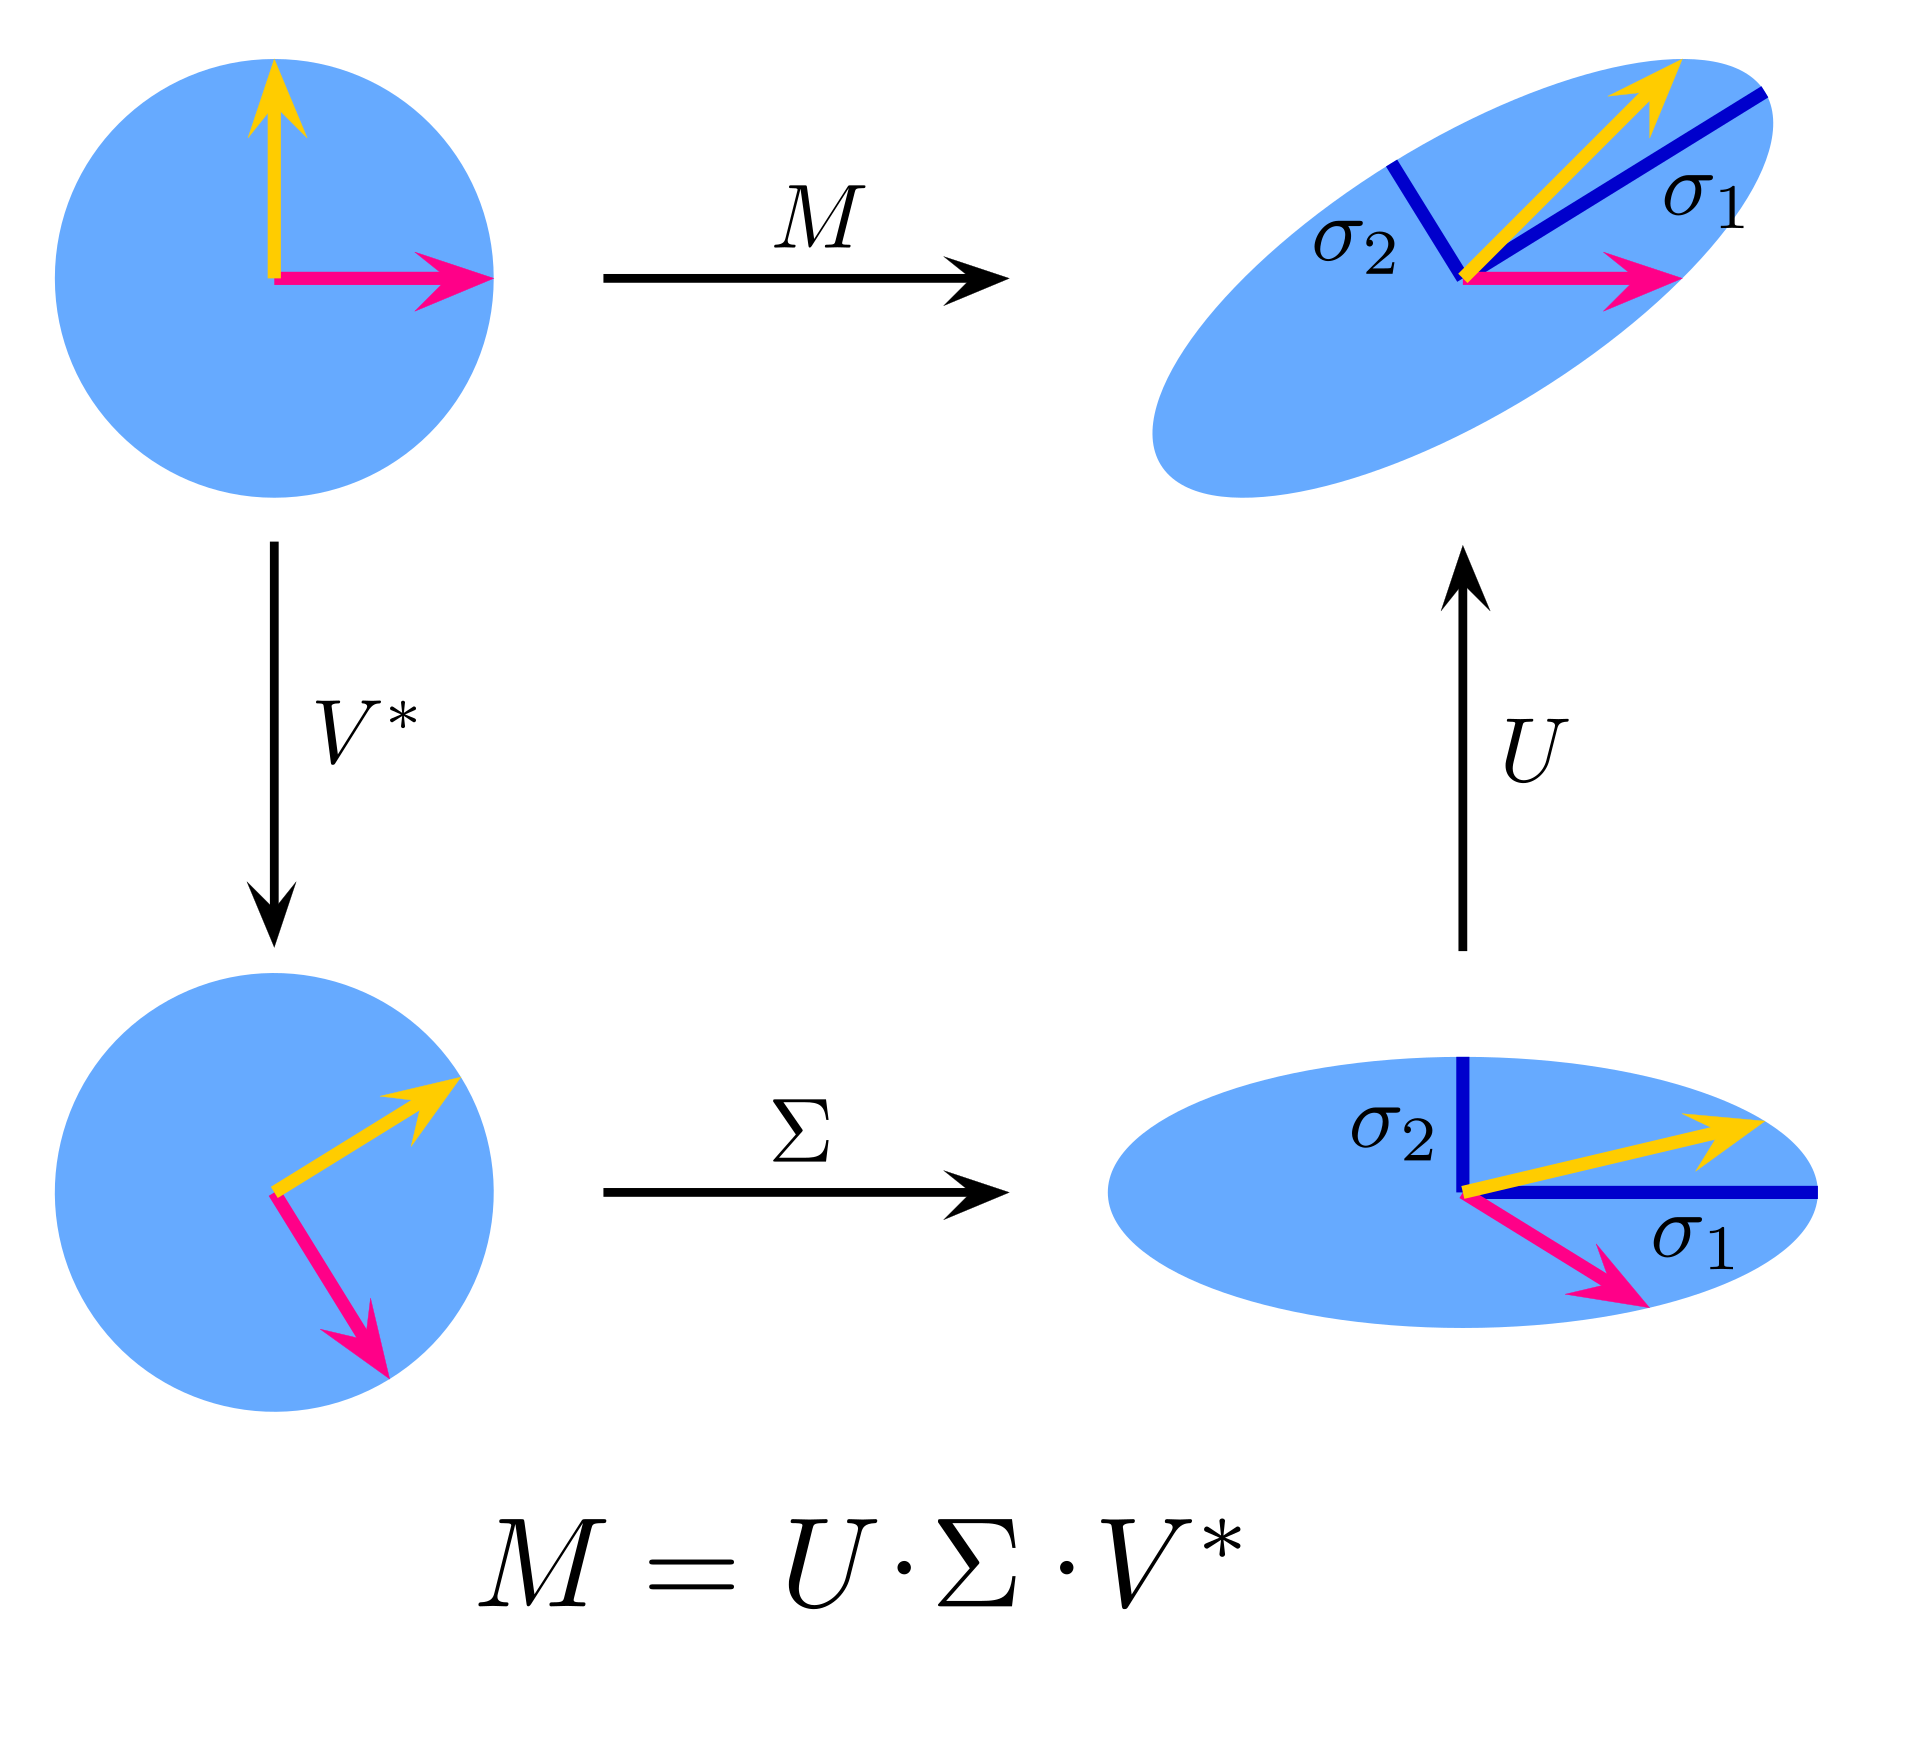
\includegraphics[width=0.4\textwidth]{lineareAlgebra/1920px-Singular-Value-Decomposition.svg.png}
    \caption*{Singulärwertzerlegung }
    \label{fig:svd}
\end{figure}

\subsubsection{Einfaches Berechnungsverfahren (über Eigenvektoren)}
\begin{enumerate}
    \item \(AA^T\) und \(A^TA\) bestimmen
    \item Für \glqq kleinere\dq Matrix aus 1) Eigenwerte \(\lambda_i\) bestimmen (char. Polynom)
    \item \(\Sigma\) mit \(diag(\sigma_1 \geq \sigma_2 \geq \hdots \geq \sigma_n)\) aufstellen; Singulärwerte \(\sigma_i = \sqrt{\lambda_i}\) auf Hauptdiagonalen; Rest \(=0\)
    \item \(U\) aufstellen: normierte Eigenvektoren für \(AA^T\) für alle \(\lambda_i\) bestimmen
    \item \(V\) aufstellen: normierte Eigenvektoren für \(A^TA\) für alle \(\lambda_i\) bestimmen; \(V^T\) bilden
\end{enumerate}



\subsubsection{Alternatives Berechnungsverfahren}

\begin{table}[H]
  \centering
  \begin{tabularx}{\textwidth}{X|l}
    %%%%%%%%%%%%%%%%%%%%%%%%%%%%%%%
    % 1. Form prüfen
    %%%%%%%%%%%%%%%%%%%%%%%%%%%%%%%
    \makecell[l]{\textbf{1. Form prüfen:} ist \(A\) \glqq hochkant\grqq? \\
        \(\rightarrow\) sonst aufwendiger zu lösen\\
        Umstellen zu \(A^T\) ist möglich, da\\
        \((A^T)^T = A\); d.h. \(A^T = V\Sigma^T U^T\)
    }
        &        
    \(A = \begin{pmatrix}       
        1 & 0 \\
        2 & 2 \\
        0 & 1
    \end{pmatrix}\)\\\\\hline

    %%%%%%%%%%%%%%%%%%%%%%%%%%%%%%%
    % 2. Eigenwerte bestimmen
    %%%%%%%%%%%%%%%%%%%%%%%%%%%%%%%
    \makecell[l]{\textbf{2. Eigenwerte von \(A^T A\) bestimmen} \\
        Eigenwerte (\(\geq 0\)) über \textit{Nullstellen char.}\\ \textit{Polynom} bestimmen,
        absteigend sortieren!
    }
        &
    \makecell[l]{            
        \(A^TA = \begin{pmatrix}       
            5 & 4 \\
            4 & 5
        \end{pmatrix}\) \\
        \(p_A(\lambda) = \det (A^T A - \lambda I) \overset{!}{=} 0\)\\
        \((5-\lambda)^2-16=0\)\\
        \(\lambda_1 = 9, \lambda_2 = 1\)
    }\\\\\hline

    %%%%%%%%%%%%%%%%%%%%%%%%%%%%%%%
    % 3. Sigma aufstellen
    %%%%%%%%%%%%%%%%%%%%%%%%%%%%%%%
    \makecell[l]{\textbf{3. \(\Sigma\) aufstellen} \\
        Diagonalmatrix mit \(\sigma_i=\sqrt[]{\lambda_i}\), Rest \(=0\)
    }
        &
    \makecell[l]{            
        \(\Sigma = \begin{pmatrix}       
            3 & 0 \\
            0 & 1 \\
            0 & 0
        \end{pmatrix}\)
    }\\\\\hline

    %%%%%%%%%%%%%%%%%%%%%%%%%%%%%%%
    % 4. Spaltenvektoren für V ermitteln
    %%%%%%%%%%%%%%%%%%%%%%%%%%%%%%%
    \makecell[l]{\textbf{4. Spaltenvektoren für \(V\) ermitteln} \\
        Eigenvektoren zu \(\lambda\) aus 2. bestimmen. Da \(A^TA\) symmetrisch\\
        ist \(\Rightarrow\) alle Eigenräume sind bereits orthogonal zueinander\\
        Wenn kein eindeutiges Ergebnis: ggf. \(v_1=1\) setzen.\\
        EV normieren und in Matrix \(V\) eintragen\\
        Für SVD: \(V^T\) bilden
    }
        &
    \makecell[l]{       
        \underline{für \(\lambda_1 = 9\):}\\     
        \(
            \left( 
            \begin{array}{cc|c}
                5 - 9 &  4 & 0\\
                4 & 5-9 & 0
            \end{array}
            \right)\Leftrightarrow 
        \)\\
        \(
            \left( 
            \begin{array}{cc|c}
                1 &  -1 & 0\\
                0 & 0 & 0
            \end{array}
            \right)\Rightarrow v_1^* = \begin{pmatrix}       
                1 \\
                1
            \end{pmatrix}
        \)\\
        \(v_1=\frac{v_1^*}{||v_1^*||} = \frac{1}{\sqrt{2}}\begin{pmatrix}
            1 \\
            1
        \end{pmatrix}\)\\\\
        \underline{für \(\lambda_2 = 1\):}\\ 
        \(\hdots\)\\
        \(v_2=\frac{v_2^*}{||v_2^*||} = \frac{1}{\sqrt{2}}\begin{pmatrix}
            -1 \\
            1
        \end{pmatrix}\)\\\\
        \(V = \frac{1}{\sqrt{2}}\begin{pmatrix}
            1 & -1 \\
            1 & 1
        \end{pmatrix}\)
    }\\\\\hline

    %%%%%%%%%%%%%%%%%%%%%%%%%%%%%%%
    % 5. U aufstellen
    %%%%%%%%%%%%%%%%%%%%%%%%%%%%%%%
    \makecell[l]{\textbf{5. \(U\) aufstellen} \\
        a) für vorhandene Singulärwerte:\\ \hspace*{1.5em}\(u_i = \frac{1}{\sigma_i}Av_i\)\\
        b) sonst: \(u_i\) so finden, dass \(u_i\) ONB sind\\
            \hspace*{1.5em}\(\rightarrow\) Kreuzprodukt (\(\mathbb{R}^3\))\\
            \hspace*{1.5em}\(\rightarrow\) Gram-Schmidt
    }
        &
    \makecell[l]{            
        \(u_1 = \frac{1}{3\sqrt{2}}\begin{pmatrix}
            1\\
            4\\
            1
        \end{pmatrix}\),
        \(u_2 = \frac{1}{\sqrt{2}}\begin{pmatrix}
            -1\\
            0\\
            1
        \end{pmatrix}\)\\
        b) \(u_3=u_1\times u_2 = \frac{1}{6}\begin{pmatrix}
            4\\
            -2\\
            4
        \end{pmatrix}\)\\
    }\\\\
    \end{tabularx}
\end{table}


\section{Mehrdimensionale Wahrscheinlichkeitsrechnung}

\subsection{Erwartungs- und Varianzrechnung}

\subsubsection{Erwartungswert}

Erwartungswert bei \underline{stetiger} Zufallsvariable \(X\) mit Dichte \(f(x)\); Lösung mit Hilfe von \emph{Integration durch Substitution} (vgl. S.~\pageref{substitution}):
\begin{equation*}
    E[g(x)]=\int_{-\infty}^{\infty}g(x)f(x)dx
\end{equation*}

Erwartungswert bei \underline{diskreter} Zufallsvariable \(X\):
\begin{equation*}
    E[g(x)]=\sum_{i=1}^{n}g(a_i)p_i = \sum_{i=1}^{n}g(a_i)P(X=a_i) 
\end{equation*}

Rechenregeln für Erwartungswerte:
\begin{itemize}
    \item \(E[aX+bY]=aE[X]+bE[Y]\)
    \item \(E[XY]=E[X]E[Y]\) \(\Leftrightarrow\) \(X\) und \(Y\) unkorreliert
    \item \(E[X^2]=Var[X]+E[X]^2\)
\end{itemize}


\subsubsection{Varianz}

Varianz bei \underline{stetiger} Zufallsvariable \(X\) mit Dichte \(f(x)\):
\begin{equation*}
    Var[X]=E[(X-E[X])^2]=E[X^2]-(E[X])^2=\int_{-\infty}^{\infty}(x-E[X])^2f(x)dx
\end{equation*}

Varianz bei \underline{diskreter} Zufallsvariable \(X\):
\begin{equation*}
    Var[X]=E[(X-E[X])^2]=\sum_{i=1}^{n}(a_i-E[X])^2p_i
\end{equation*}

Rechenregeln für Varianzen:
\begin{itemize}
    \item \(Var[aX+bY]=a^2Var[X]+b^2Var[Y]+2abCov[X,Y]\)
    \item \(Var[X+Y]=Var[X]+Var[Y]+2Cov[X,Y]\)
\end{itemize}



\subsubsection{Kovarianz, Korrelation}
\begin{equation*}
    Cov[X,Y]=E[(X-E[X])(Y-E[Y])]=E[XY]-E[X]E[Y]
\end{equation*}

\begin{equation*}
    Cov[X,Y]=Cov[Y,X] \text{ und } Cov[X,X]=Var[X]
\end{equation*}

\begin{equation*}
    r_{XY} = Cor[X,Y]=\frac{Cov[X,Y]}{\sqrt{Var(X)Var(Y)}} \rightarrow [-1;+1]
\end{equation*}

Zusammenhänge beachten: 
\begin{itemize}
    \item statistische Unabhängigkeit \(\Rightarrow\) Unkorreliertheit
    \item Unkorreliertheit \(\Rightarrow\) statistische Unabhängigkeit, \underline{nur} wenn \(X\) und \(Y\) normalverteilt sind
\end{itemize}

\subsubsection{Linearkombinationen}
\begin{equation*}
    E[aX+bY]=aE[X]+bE[Y]
\end{equation*}

\begin{equation*}
    Var[aX+bY]=a^2Var[X]+b^2Var[Y]+2abCov[X,Y]
\end{equation*}

\begin{equation*}
    Var[X_1 + \hdots + X_n]=\sum_{i=1}^{n}Var[X_i] + 2\sum_{1\leq i<j\leq n}Cov[X_i,X_j] \rightarrow\text{ \emph{Satz von Bienaymé}}
\end{equation*}

\subsubsection{Mengen}

\begin{figure}[ht]
    \centering
    \begin{minipage}{.5\textwidth}
      \centering
      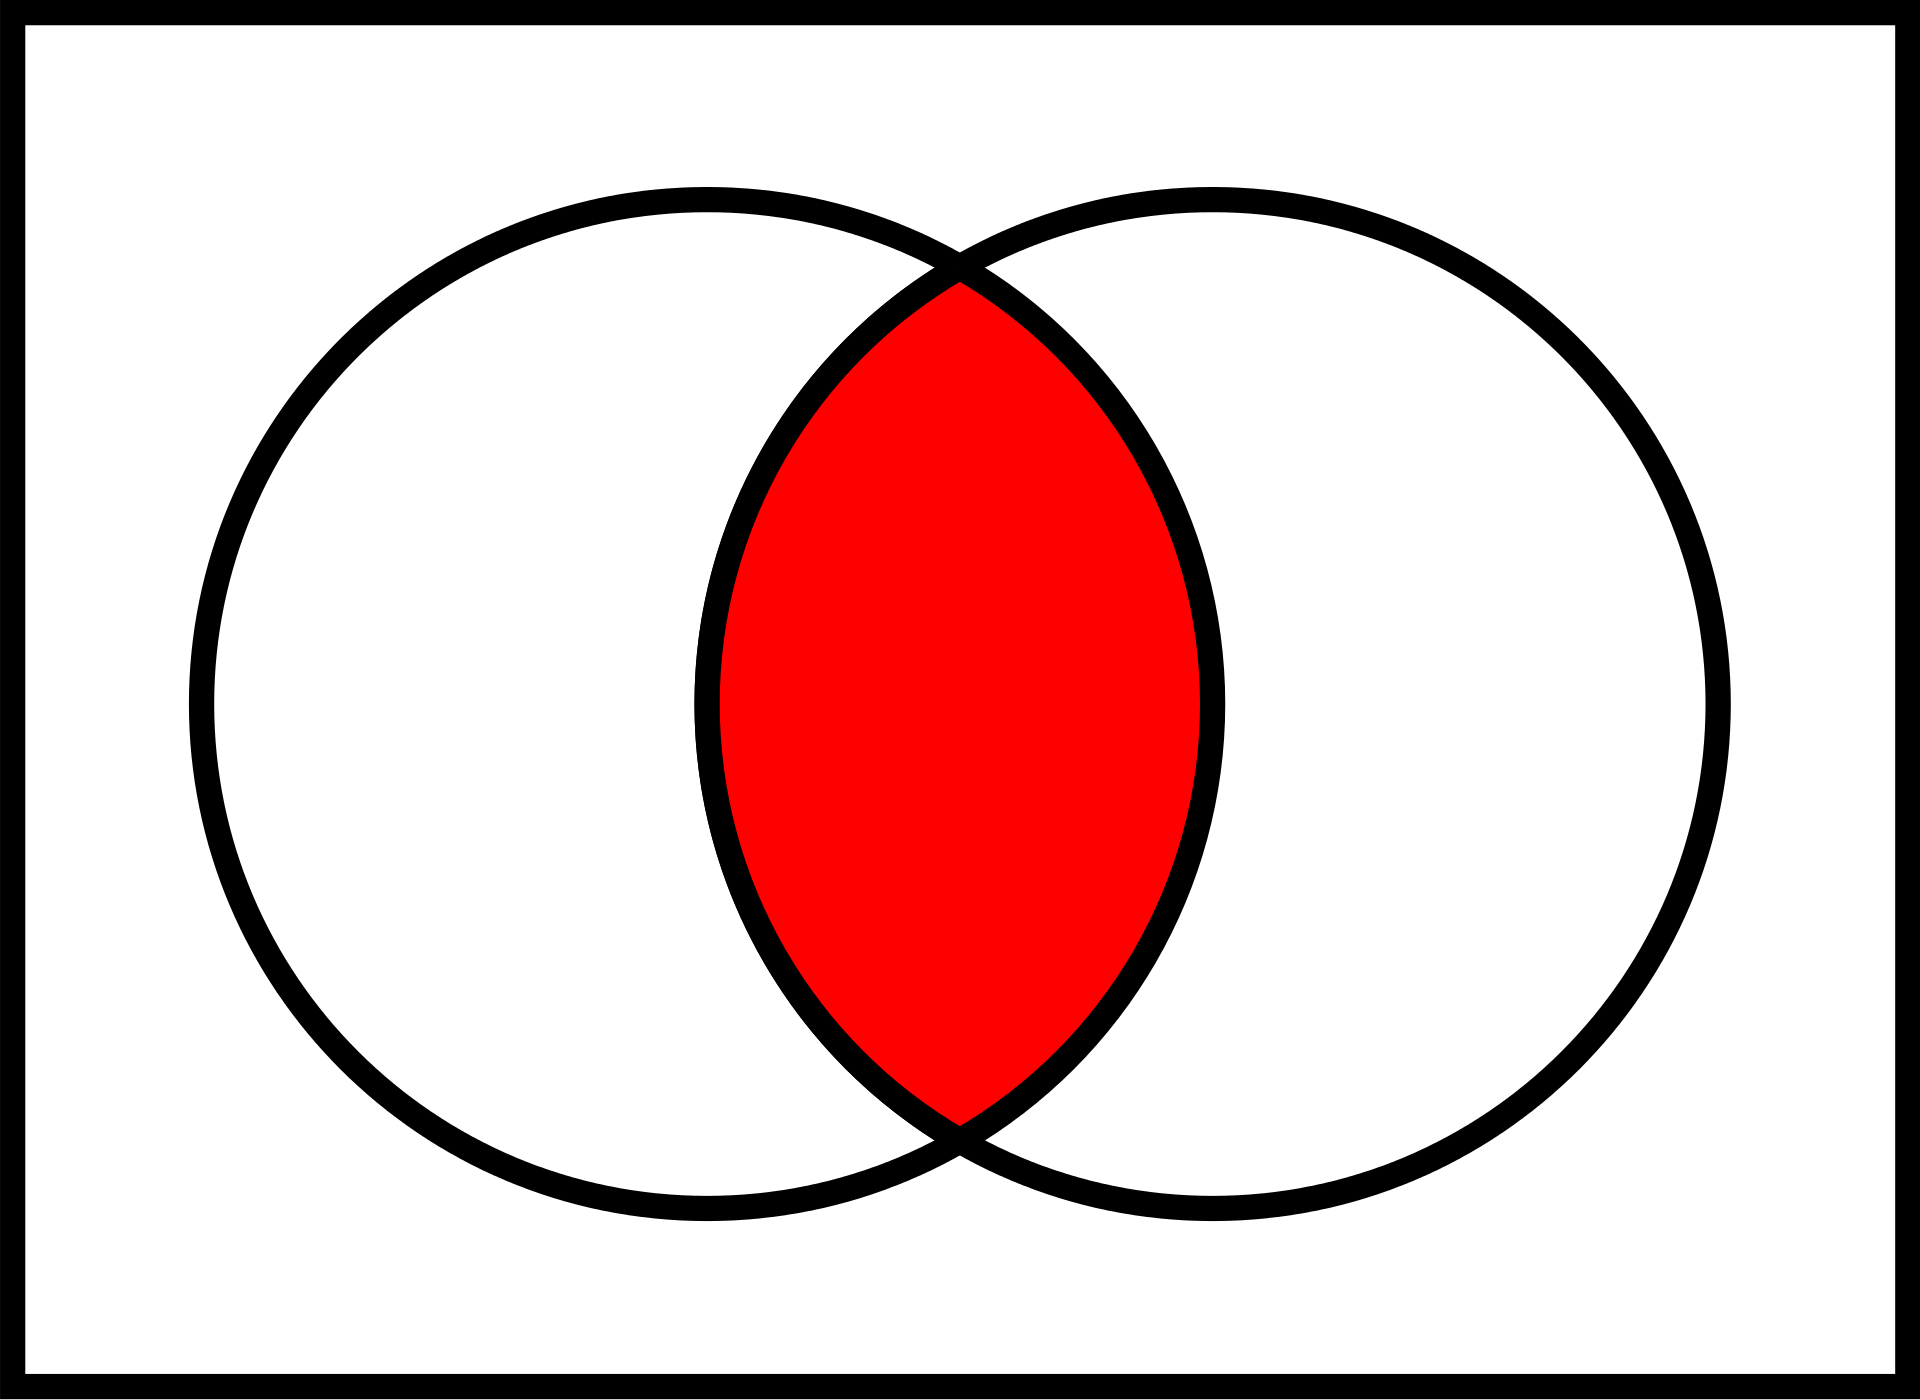
\includegraphics[width=.4\linewidth]{mehrdimWktrechnung/Venn0001.svg.png}
      \captionof*{figure}{Schnittmenge \(A\cap B\)}
      \label{fig:schnittmenge}
    \end{minipage}%
    \begin{minipage}{.5\textwidth}
      \centering
      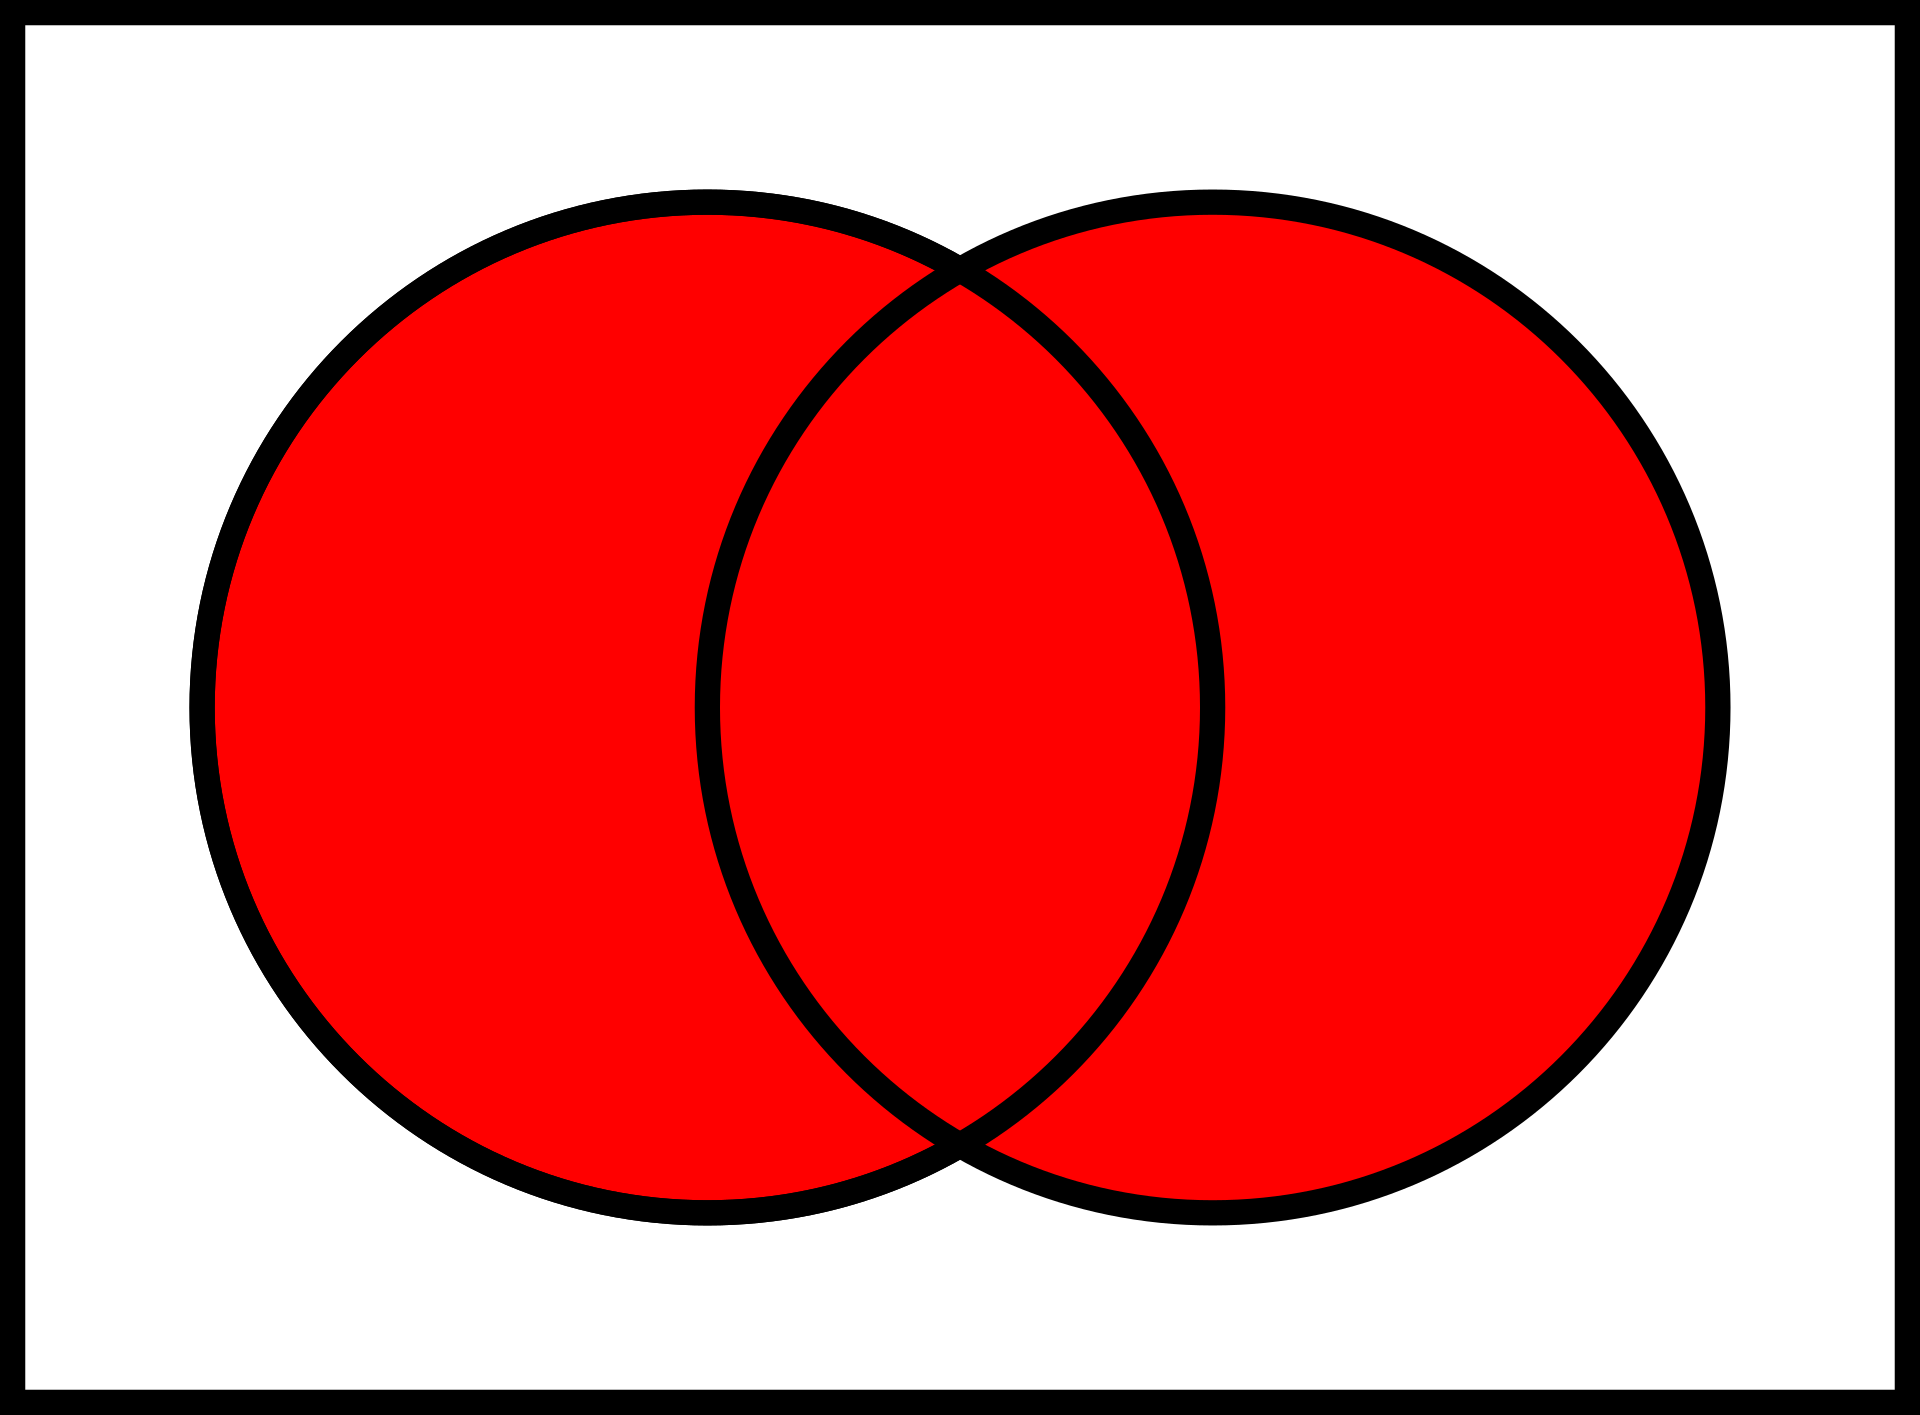
\includegraphics[width=.4\linewidth]{mehrdimWktrechnung/Venn0111.svg.png}
      \captionof*{figure}{Vereinigung \(A\cup B\)}
      \label{fig:vereinigungsmenge}
    \end{minipage}
\end{figure}

\begin{equation*}
    A\cup B = A+B-A\cap B
\end{equation*}

\begin{equation*}
    A = (A\cap B) \cup (A\cap B^c)
\end{equation*}

\subsubsection{Konvergenz}

\begin{itemize}
    \item \textbf{in Wahrscheinlichkeit}: \(X_n \xrightarrow{P} X\) wenn \(\forall \epsilon > 0: \lim_{n\rightarrow\infty}P(|X_n-EW(X)| \geq\epsilon)=\\=P(X_n \geq\epsilon)=P(X_1\geq\epsilon)\times \hdots \times P(X_n\geq\epsilon)=(1-\epsilon)^n = 0\) für \(X_n\) unab. und gleichverteilt in [0,1]
    \item \textbf{im p-ten Mittel/in \(\mathcal{L}^p\)}: \(X_n \xrightarrow{\mathcal{L}^p} X\) wenn \(\lim_{n\rightarrow\infty}E(|X_n-X|^p)\)
    \item \textbf{fast sicher}: \(X_n \xrightarrow{fs} X\) wenn \(P(\lim_{n\rightarrow\infty}X_n=X)=1\)
\end{itemize}

Konvergenz bei
\begin{itemize}
    \item einer \underline{Summe} von Zufallsvariablen: \(X_n \rightarrow a\) und \(Y_n \rightarrow b \Longrightarrow X_n + Y_n \rightarrow a + b\)
    \item einem \underline{Produkt} von Zufallsvariablen: \(X_n \xrightarrow{\mathbb{P}} X\) und \(Y_n \xrightarrow{\mathbb{P}} Y \Longrightarrow X_nY_n \xrightarrow{\mathbb{P}} XY\)
\end{itemize}

Zusammenhang zwischen Konvergenzarten: Wenn \(X_n \xrightarrow{f.s.} X\) oder \(X_n \xrightarrow{\mathcal{L}^p} X\), dann \(X_n \xrightarrow{\mathbb{P}} X\)


\subsection{Bedingte Wahrscheinlichkeit, Bayes-Theorem}

\begin{minipage}{0.50\textwidth}
    \begin{equation*}
        P(A|B)=\frac{P(A\cap B)}{P(B)}
    \end{equation*}
\end{minipage}
\hspace{1cm}
\begin{minipage}{0.50\textwidth}
    \begin{equation*}
        P(A|B)=\frac{P(B|A)P(A)}{P(B)}
    \end{equation*}
\end{minipage}


\section{Optimierung}


\subsection{Konvexe Funktionen/Mengen}


Eine \emph{Menge} $G \subseteq \mathbb{R}^n$ heißt \emph{konvex}, wenn für alle $x, y \in G$ und $t \in [0, 1]$ gilt:
\begin{equation*}
t x + (1 - t) y \in G
\end{equation*}
D.h. die Verbindungsstrecke zwischen zwei Punkten der Menge liegt komplett in der Menge.
\\
\\
Eine \emph{Funktion} $f: \mathbb{R}^n \rightarrow \mathbb{R}$ heißt \emph{konvex} (\(\leq\)) bzw. \emph{strikt konvex} (\(<\)), wenn für alle $x, y \in \mathbb{R}^n$ und $t \in [0, 1]$ gilt:
\begin{equation*}
    f(t x + (1 - t) y) \leq t f(x) + (1 - t) f(y)
\end{equation*}

\underline{Vorgehensweise:}

\begin{enumerate}
    \item Hesse-Matrix (\(H_f(x)\), =symmetrisch) bestimmen:
            \(H_f(x) =
                \begin{pmatrix}
                    f_{xx} & f_{xy} \\
                    f_{yx} & f_{yy}
                \end{pmatrix}
            \)
    \item Definitheit bestimmen:
        \begin{enumerate}
            \item über \emph{Eigenwerte}
                \begin{itemize}
                    \item Nullstellen charakteristisches Polynom bestimmen (\(\rightarrow \) \ref{sec:charPolynom})
                    \item Interpretation:
                    \begin{itemize}
                        \item alle \(\lambda>0\rightarrow H_f(x)=\) pos. definit
                        \item alle \(\lambda\geq 0\rightarrow H_f(x)=\) pos. semidefinit 
                        \item alle \(\lambda<0\rightarrow H_f(x)=\) neg. definit 
                        \item alle \(\lambda\leq 0\rightarrow H_f(x)=\) neg. semidefinit 
                        \item \(\lambda\) positiv und negativ \(\rightarrow H_f(x)=\) indefinit
                    \end{itemize}
                \end{itemize}
            \item über \emph{Diagonaldominanz}: Ist \(H_f(x)\) Diagonaldominant und alle Diagonalelemente \(>0\), so ist \(H_f(x)\) positiv definit.\\
                \(\rightarrow \) für alle Zeilen: \(||\)Diagonalelement\(|| > \sum ||\)übrige Zeilenelemente\(||\) 
            \item \emph{Choleskyzerlegung} ist möglich \(= H_f(x)\) ist positiv definit
        \end{enumerate}
    \item Konvexität bestimmen:
        \begin{itemize}
            \item \(H_f(x)\) positiv definit \(\Leftrightarrow\) \(f\) strikt konvex
            \item \(H_f(x)\) positiv semidefinit \(\Leftrightarrow\) \(f\) konvex
            \item \(H_f(x)\) negativ definit \(\Leftrightarrow\) \(f\) strikt konvex
            \item \(H_f(x)\) negativ semidefinit \(\Leftrightarrow\) \(f\) konvex
        \end{itemize}
\end{enumerate}

\subsection{Optimierung ohne Nebenbedingungen}

\subsection{Optimierung ohne NB - Gradientenverfahren}
Beginnend an einer Stelle \(x_0\): 
\begin{enumerate}
\item Berechne Gradienten \(\nabla f(x_n)\) (im ersten Schritt mit \(x_0\))
\item Setze \(x_{n+1} = x_n - \alpha \nabla f(x_n), \;\;\;\; n \geq 0\) mit Schrittweite \(\alpha\)
\item Wiederhole Schritt 1 und 2 bis Abbruchkriterium erfüllt; \(x^* = x_k\)
\end{enumerate}

Approximation von \(\nabla f(x_0)\) durch \(\frac{f(x_n) - f(x_{n-1})}{x_n - x_{n-1}}\) möglich.

\subsubsection{Newton-Verfahren}

\subsection{Optimierung unter Nebenbedingungen}
Lagrangemultiplikatoren\\
Dualität\\
KKT-Bedingungen
\section{Statistik}

\subsection{Verteilungen}
\label{verteilungen}

\subsubsection{Binomialverteilung (\(X\sim Bin(n,\pi)\))}
Diskrete Wahrscheinlichkeitsverteilung; beschreibt die Anzahl an Erfolgen in einer Serie von unabhängigen Versuchen, die jeweils genau zwei Ergebnisse haben (Erfolg/Misserfolg); z.B. beim Münzwurf, Ziehen mit Zurücklegen.

\begin{itemize}
    \item \(n\)=Anzahl der Versuche/Ziehungen (beeinflusst \emph{Breite} der Verteilung), \(\pi\)=Erfolgswahrscheinlichkeit (z.B. \(0.3\); beeinflusst Schiefe der Verteilung)
    \item \textbf{Wahrscheinlichkeit:} \(P(X=k)=\binom{n}{k}\pi^k(1-\pi)^{n-k}\); \(k=\) Anzahl der gewünschten Erfolge
    \item \textbf{Erwartungswert:} \(E(X)=n\pi\)
    \item \textbf{Varianz:} \(Var(X)=n\pi(1-\pi)\)
    \item \textbf{Normalapproximation:} \(X\sim N(n\pi, n\pi(1-\pi))\)
    \item \textbf{Binomialkoeffizient:} \(\binom{n}{k}=\frac{n!}{k!(n-k)!}\)
    \item \textbf{Bernoulli-Verteilung:} Spezialfall der Binomialverteilung mit \(n=1\)
\end{itemize}


\subsubsection{Poisson-Verteilung (\(X\sim Poi(\mu)\))}
Diskrete Wahrscheinlichkeitsverteilung; beschreibt die Anzahl an Ereignissen in einem festgelegten Zeitintervall, wenn die Ereignisse mit einer konstanten Rate und unabhängig von der Zeit auftreten; z.B. Anzahl der Anrufe in einer Stunde, Anzahl der Kunden in einer Schlange, Anzahl der Fehler in einem Text. Für kleine \(\mu\) zeigt die Poisson-Verteilung eine starke Asysmmetrie (Rechtsschiefe).

\begin{itemize}
    \item \(\varTheta \)=Erwartungswert (z.B. \(0.3\))
    \item \textbf{Wahrscheinlichkeit:} \(P(X=n)=\frac{\varTheta^n}{n!}e^{-\varTheta}\); \(n=\) Anzahl der gewünschten Ereignisse
    \item \textbf{Erwartungswert:} \(E(X)=\varTheta\)
    \item \textbf{Varianz:} \(Var(X)=\varTheta\)
    \item \textbf{Normalapproximation:} \(X\sim N(\varTheta, \varTheta)\)
\end{itemize}


\subsubsection{Hypergeometrische Verteilung (\(X\sim H(n,N,m)\))}

Ähnlich wie Binomialverteilung, aber ohne Zurücklegen; z.B. beim Ziehen ohne Zurücklegen aus einer Urne mit \(N\) Kugeln, davon \(m\) mit Erfolgsmarkierung.

\begin{itemize}
    \item \(n\)=Anzahl der Versuche/Ziehungen, \(N\)=Anzahl der Kugeln in der Urne, \(m\)=Anzahl der Kugeln mit Erfolgsmarkierung
    \item \textbf{Wahrscheinlichkeit:} \(P(X=k)=\frac{\binom{m}{k}\binom{N-m}{n-k}}{\binom{N}{n}}\); \(k=\) Anzahl der gewünschten Erfolge
    \item \textbf{Erwartungswert:} \(E(X)=n\frac{m}{N}\)
    \item \textbf{Varianz:} \(Var(X)=n\frac{m}{N}\left(1-\frac{m}{N}\right)\left(\frac{N-n}{N-1}\right)\)
    \item \textbf{Normalapproximation:} \(X\sim N\left(n\frac{m}{N}, n\frac{m}{N}\left(1-\frac{m}{N}\right)\left(\frac{N-n}{N-1}\right)\right)\)
\end{itemize}


\subsubsection{Normalverteilung (\(X\sim N(\mu, \sigma^2)\))}
Stetige Wahrscheinlichkeitsverteilung; beschreibt viele natürliche Vorgänge (z.B. Körpergröße, IQ, Fehler in Messungen); zentrales Grenzwerttheorem: Summe von unabhängigen Zufallsvariablen strebt gegen Normalverteilung; symmetrisch um \(\mu\), \(\sigma^2\)-bestimmte Breite; \(\mu\)=Erwartungswert, \(\sigma^2\)=Varianz, \(\sigma\)=Standardabweichung.\\

\begin{minipage}{0.5\textwidth}
    \begin{itemize}
        \item \textbf{Erwartungswert:} \(E(X)=\mu\)
        \item \textbf{Varianz:} \(Var(X)=\sigma^2\)
        \item \textbf{Standardnormalverteilung:} \(Z\sim N(0,1)\)
    \end{itemize}
\end{minipage}
\begin{minipage}{0.2\textwidth}
    \underline{Dichtefunktion}:
    \begin{equation*}
        f(x)=\frac{1}{\sqrt{2\pi\sigma^2}}e^{-\frac{(x-\mu)^2}{2\sigma^2}}
    \end{equation*}
\end{minipage}
\hspace{1cm}
\begin{minipage}{0.2\textwidth}
    \underline{\(X\sim N(0, 1)\)}:
    \begin{equation*}
        \varphi(x)=\frac{1}{\sqrt{2\pi}}e^{-\frac{x^2}{2}}
    \end{equation*}
\end{minipage}

\input{statistik/parameterschätzung}

\subsection{Zentraler Grenzwertsatz}

Der zentrale Grenzwertsatz besagt, dass die Summe von unabhängigen, identisch verteilten Zufallsvariablen einer beliebigen Verteilung für \(n\rightarrow\infty\) gegen eine Normalverteilung konvergiert, auch wenn die Ausgangsverteilung nicht normalverteilt ist. Als Theorem mit \underline{E}rwartungswert (\(\mu\)), \underline{V}arianz (\(\sigma^2\)) und \(n\) Zufallsvariablen:\\


\begin{equation*}
    \lim_{n\rightarrow\infty} P\left(\frac{\sum_{i=1}^{n}X_i - n\mu}{\sigma\sqrt{n}}\leq x\right) = \sqrt{\frac{n}{V}}\left(\frac{1}{n}\sum_{i=1}^{n}X_i-E\right) \rightarrow \Phi(x) \sim N(0,1)   
\end{equation*}

\subsection{Regression}

Unterscheidung zwischen (einfacher/multipler) linearer und logistischer Regression:

\begin{itemize}
    \item \textbf{Lineare Regression:}
    \begin{itemize}
        \item Ziel: Schätzung des Erwartungswerts einer abhängigen Variable \(Y\) in Abhängigkeit von einer oder mehreren unabhängigen Variablen \(X\)
        \item Modell: \(Y = \beta_0 + \beta_1 \cdot X_1 + \beta_2 \cdot X_2 + \ldots + \beta_n \cdot X_n + \varepsilon\)
        \item \(\varepsilon\): Fehlerterm
        \item \(\beta_0\): Achsenabschnitt
        \item \(\beta_1, \beta_2, \ldots, \beta_n\): Regressionskoeffizienten
    \end{itemize}
    \item \textbf{Logistische Regression:}
    \begin{itemize}
        \item Ziel: Schätzung der Wahrscheinlichkeit, dass eine abhängige Variable \(Y\) den Wert 1 annimmt, in Abhängigkeit von einer oder mehreren unabhängigen Variablen \(X\)
        \item Modell: \(P(Y=1) = \frac{1}{1+e^{-(\beta_0 + \beta_1 \cdot X_1 + \beta_2 \cdot X_2 + \ldots + \beta_n \cdot X_n)}}\)
        \item \(\beta_0, \beta_1, \beta_2, \ldots, \beta_n\): Regressionskoeffizienten
    \end{itemize}
\end{itemize}

\subsection{Konfidenzintervalle}

Schätzung eines Intervalls, in dem sich der wahre Wert (z.B. der Erwartungswert~\(\mu\)) mit einer gewissen Wahrscheinlichkeit befindet.

\subsubsection{Vorgehensweise bei Normalverteilung und \textbf{bekanntem} \boldmath{\(\sigma\)}}

\begin{enumerate}
    \item Punktschätzung des Erwartungswerts aus \(n\) Stichproben (\(x_i\))
            \[M(x)=\frac{1}{n}\sum_{i=1}^{n}x_i\]\\
            \(\rightarrow\) dieser entspricht i.d.R. nicht dem wahren Wert \(\mu\) der Grundgesamtheit.

    \item Konfidenzniveau (\(1-\alpha\); \(\alpha=\) Irrtumsniveau) festlegen und \(z_{1-\frac{\alpha}{2}}\) aus Tabelle zur Normalverteilung ablesen
        \begin{itemize}
            \item \(90\% = 1-\alpha \rightarrow \alpha=0.1\rightarrow z_{0.95}=1.65\)
            \item \(95\% \rightarrow \alpha=0.05\rightarrow z_{0.975}=1.96\)
            \item \(96\% \rightarrow \alpha=0.04\rightarrow z_{0.980}=2.06\)
            \item \(97\% \rightarrow \alpha=0.03\rightarrow z_{0.985}=2.17\)
            \item \(98\% \rightarrow \alpha=0.02\rightarrow z_{0.99}=2.33\)
            \item \(99\% \rightarrow \alpha=0.01\rightarrow z_{0.995}=2.58\)
        \end{itemize}
    \item Berechnung des Konfidenzintervalls
        \begin{equation*}
            \mathcal{I}(x) = \left[M(x) - z_{1-\frac{\alpha}{2}} \cdot \frac{\sigma}{\sqrt{n}}\hspace{0.5em}; \hspace{0.5em}M(x) + z_{1-\frac{\alpha}{2}} \cdot \frac{\sigma}{\sqrt{n}}\right]
        \end{equation*}
        \emph{ist ein Konfidenzintervall zum Sicherheitsniveau \(1-\alpha\)}\\
\end{enumerate}

\subsubsection{Vorgehensweise bei Normalverteilung und \textbf{unbekanntem} \boldmath{\(\sigma\)}}

Grds. analog zu oben, wobei Werte für \(t_{n-1,1-\frac{\alpha}{2}}\) aus der t-Verteilung verwendet werden (Studentsche (\(t\)-) Verteilung mit \(n-1\) Freiheitsgraden).  Nur bei \(n\geq 30\).

\begin{enumerate}
    \item Punktschätzung des Erwartungswerts aus \(n\) Stichproben (\(x_i\))
            \[M(x)=\frac{1}{n}\sum_{i=1}^{n}x_i\]\\
            \(\rightarrow\) dieser entspricht i.d.R. nicht dem wahren Wert \(\mu\) der Grundgesamtheit.
    \item Berechnung des Standardfehlers der Stichprobenmittelwerte
        \[\text{korrigierte Stichprobenvarianz: }V^*(x)=\frac{1}{n-1}\sum_{i=1}^{n}(x_i-M(x))^2\]
        \[\text{Standardfehler: }s^*=\sqrt{\frac{V^*(x)}{n}}\]
        \(\rightarrow\) dieser entspricht i.d.R. nicht dem wahren Wert \(\sigma\) der Grundgesamtheit.
    \item Berechnung des Konfidenzintervalls
    \begin{equation*}
        \mathcal{I}(x) = \left[M(x) - t_{n-1;1-\frac{\alpha}{2}} \cdot s^*\hspace{0.5em}; \hspace{0.5em}M(x) + t_{n-1;1-\frac{\alpha}{2}} \cdot s
        ^*\right]
    \end{equation*}
    \emph{ist ein Konfidenzintervall zum Sicherheitsniveau \(1-\alpha\) mit \(n-1\) Freiheitsgraden}\\
\end{enumerate}

\subsubsection{Vorgehensweise im Binominalmodell}

Wenn X binominalverteilt ist (\(X \sim  B(n, \pi)\), \(n\)=Anzahl gezogene Versuche, \(\pi\)=Erfolgswahrscheinlichkeit), \(n\) groß und die Varianz nicht zu klein ist (Faustregel: \(n\pi(1-\pi) > 9\)), gilt die Approximation durch die Normalverteilung mit:

\begin{itemize}
    \item Erwartungswert: \(\mu=n\pi\)
    \item Standardabweichung: \(\sigma=\sqrt{n\pi(1-\pi)}\)
    \item Standardfehler: \(s=\sqrt{\frac{\pi(1-\pi)}{n}}\)
    \item Punktschätzung: \(\hat{\pi}=\frac{x}{n}\)
    \item Konfidenzintervall für \(\pi\): \(\mathcal{I}(\pi)\approx \left[\hat{\pi}-z_{1-\frac{\alpha}{2}}\cdot s; \hat{\pi}+z_{1-\frac{\alpha}{2}}\cdot s\right]\)
    \item Konfidenzintervall für \(\mu\): \(\mathcal{I}(\mu)\approx \left[\hat{\mu}-z_{1-\frac{\alpha}{2}}\cdot s; \hat{\mu}+z_{1-\frac{\alpha}{2}}\cdot s\right]\)
\end{itemize}

\subsection{Tests}

\begin{itemize}
    \item \textbf{Nullhypothese (\(H_0\)):} Annahme, die geprüft werden soll (z.B. \(H_0: p_0=0.3\) als EW für Münzwurf)
    \item \textbf{Gegenhypothese (\(H_1\)):} Gegenteil der Nullhypothese
        \begin{itemize}
            \item Alternativtest: Prüfe, ob anstatt \(H_0: p_0=0.3\) nicht \(H_1: p_1=0.2\) gilt
            \item Linksseitiger Test: Prüfe, ob anstatt \(H_0: p_0=0.3\) nicht \(H_1: p_1<0.3\) gilt
            \item Rechtsseitiger Test: Prüfe, ob anstatt \(H_0: p_0=0.3\) nicht \(H_1: p_1>0.3\) gilt
            \item Zweiseitiger Test: Prüfe, ob anstatt \(H_0: p_0=0.3\) nicht \(H_1: p_1\neq0.3\) gilt
        \end{itemize}
    \item \textbf{Signifikanzniveau (\(\alpha\)):} Auch: Niveau des Testverfahrens. (Irrtums-)Wahrscheinlichkeit, mit der die Nullhypothese fälschlicherweise abgelehnt wird
    \item \textbf{Teststatistik:} Funktion der Stichprobenwerte, die zur Entscheidung über die Annahme oder Ablehnung der Nullhypothese herangezogen wird
    \item \textbf{Ablehnungsbereich:} Bereich der Teststatistik, in dem die Nullhypothese abgelehnt wird
    \item \textbf{p-Wert:} Wahrscheinlichkeit, mit der die Nullhypothese verworfen werden kann
    \item \textbf{Fehler 1. Art:} \(H_0\) wird fälschlicherweise abgelehnt
    \item \textbf{Fehler 2. Art:} \(H_0\) wird fälschlicherweise nicht abgelehnt
\end{itemize}


\subsubsection{\(\chi^2\)-Anpassungstest}

Vergleicht die beobachtete Verteilung einer Stichprobe mit 
einer theoretischen (erwarteten) Verteilung. Es wird geprüft, 
ob die beobachtete Häufigkeitsverteilung von Kategorien mit der 
erwarteten Häufigkeitsverteilung übereinstimmt (z.B. ob beobachtete erste Ziffern der \emph{Benford-Verteilung} (\(\mathbb{P}(X\in E_i) = \log_{10}(1+1/i)\)) entsprechen).\\

\textbf{1. Voraussetzung:} Zufallsvariable \(X\) (z.B. Ergebnis eines Würfelwurfs) mit \(s\) Ausprägungen 
(Kategorien; z.B. 1-6 Würfelaugen) und \(N\) Beobachtungen (Stichprobenumfang); Mindestens: \(N\geq 5 / \min(\rho_i)\)\\

\textbf{2. Nullhypothese (\(H_0\)):} Die tatsächliche Verteilung entspr. der erwarteten Verteilung (\(P(X \in A_i)=\rho_i=\frac{1}{6}\))\\

\textbf{3. Gegenhypothese (\(H_1\)):} Nicht \(H_0\)\\

\textbf{4. \(\chi^2\)-Teststatistik:}

\begin{equation*}
    D_{\rho} = \sum_{i=1}^{s}\frac{(h(i)-N\rho(i))^2}{N\rho(i)}=\left(\sum_{i=1}^{s}\frac{h(i)^2}{N\rho(i)}\right)-N=N\left(\sum_{i=1}^{s}\frac{L(i)^2}{\rho(i)}\right) - N
\end{equation*}
wobei
\begin{itemize}
    \item \(N\) = Stichprobengröße \emph{(z.B. 50 Würfe mit Würfel)}
    \item \(s\) = Anzahl der Kategorien \emph{(z.B. 6 Würfelaugen)}
    \item \(A_i\) = Kategorie \(i\) \emph{(z.B. Würfelaugen 1-6)}
    \item \(h(i)\) = Anzahl der Beobacht. in Kategorie \(A_i\) \emph{(z.B. 8 Würfe 1er Würfe)}
    \item \(L(i)=\frac{h(i)}{N}\) = relative Häufigkeit der Beobachtungen in Kategorie \(A_i\) \emph{(z.B. 8/50 Würfe mit Würfelaugen 1 usw.)}
    \item \(\rho(i)\) = Wahrscheinlichkeit der Kategorie \(A_i\) \emph{(z.B. \(\frac{1}{6}\) für Würfelauge 1 usw.)}
    \item \(\alpha\) = Irrtumswahrscheinlichkeit/Signifikanzniveau \emph{(z.B. 5\%)}
\end{itemize}

\textbf{5. Ablehnungsbereich:} \(H_0\) ablehnen, wenn:  \(D_{\rho} > \chi^2_{s-1;1-\alpha}\)\\


Wenn nach einem \textbf{\(p\)-Wert} gefragt wird: Hierbei sucht man rückwärts in der Tabelle den Eintrag, der gerade so noch kleiner ist als der in der Aufgabe genannte Wert. Der Wert in der Spalte \(\alpha\) ist dann der gesuchte \(p\)-Wert. Dieser gibt das größte Signifikanzniveau an, bei dem die Nullhypothese verworfen wird. Je kleiner der \(p\)-Wert, desto unwahrscheinlicher ist es, dass die beobachteten Daten unter der Nullhypothese vorkommen könnten.\\

\subsubsection{\(\chi^2\)-Unabhängigkeitstest}

Prüft die Unabhängigkeit zweiter Merkmale, d.h. ob das Vorkommen einer Variable von der anderen ahängt oder nicht.\\


\textbf{1. Voraussetzung:} Zufallsvariable \(X\) und \(Y\) nehmen jeweils zwei Werte an (z.B. \(X\)=männlich/weiblich, \(Y\)=raucht/nicht raucht).\\

\textbf{2. Nullhypothese (\(H_0\)):} \(X\) und \(Y\) sind stochastisch unabhängig\\

\textbf{3. Gegenhypothese (\(H_1\)):} Nicht \(H_0\)\\

\textbf{4. \(\chi^2\)-Teststatistik:}\\

Aufstellen einer Vierfeldertafel:\\

\begin{minipage}[c]{.4\textwidth}
    \centering
    \begin{tabular}{c|c|c|c}
                   & $Y$           & $\overline{Y}$ & $\Sigma$         \\ 
                   \hline
    $X$            & \(N_{11}\)    & \(N_{12}\)     & \(N_{1 \cdot} \) \\ 
    \hline
    $\overline{X}$ & \(N_{21}\)    & \(N_{22}\)     & \(N_{2\cdot} \)  \\ 
    \hline
    $\Sigma$       & $N_{\cdot 1}$ & $N_{\cdot 2}$  & $n$
    \end{tabular}
\end{minipage}
\begin{minipage}[c]{.6\textwidth}
    \centering
    \begin{tabular}{c|c|c|c}
             & Nichtraucher & Raucher & $\Sigma$ \\ 
    \hline
    männlich & 170          & 30      & 200 \\
    \hline
    weiblich & 250          & 150     & 400  \\
    \hline
    $\Sigma$ & 420          & 180     & 600
    \end{tabular}
\end{minipage}\\\\

Daraus Berechnung der Teststatistik:
\begin{equation*}
    D_{\rho} = n \frac{(N_{11}N_{22}-N_{12}N_{21})^2}{N_{1\cdot}N_{2\cdot}N_{\cdot1}N_{\cdot2}}
\end{equation*}

\emph{Gedankenstütze: Determinante hoch 2 geteilt durch Produkt aus allen Spalten- und Zeilensummen}\\

\textbf{5. Ablehnungsbereich:} \(H_0\) ablehnen, wenn:  \(T > \chi^2_{1;1-\alpha}\)\\
\section{Markov-Ketten}
	
\begin{center}
	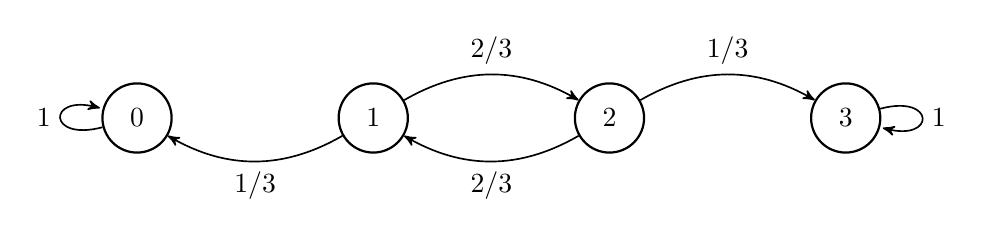
\begin{tikzpicture}[->, >=stealth', auto, semithick, node distance=3cm]
	\tikzstyle{every state}=[fill=white,draw=black,thick,text=black,scale=1]
	\node[state]    (A)                     {$0$};
	\node[state]    (B)[right of=A]   {$1$};
	\node[state]    (C)[right of=B]   {$2$};
	\node[state]    (D)[right of=C]   {$3$};
	\path
	(A) edge[loop left]			node{$1$}	(A)
	(B) edge[bend left,below]	node{$1/3$}	(A)
	edge[bend left,above]		node{$2/3$}	(C)
	(C) edge[bend left,below]	node{$2/3$}	(B)
	edge[bend left,above]		node{$1/3$}	(D)
	(D) edge[loop right]		node{$1$}	(D);
	%\node[above=0.5cm] (A){Patch G};
	%\draw[red] ($(D)+(-1.5,0)$) ellipse (2cm and 3.5cm)node[yshift=3cm]{Patch H};
	\end{tikzpicture}
\end{center}

\subsection{Übergangsmatrix}

\begin{itemize}
	\item Zeilen: Quelle, von diesem Knoten startet man
	\item Spalten: Zielknoten
	\item \(p_{ij}\) gibt dann die Übergangswahrscheinlichkeiten an
	\begin{itemize}
		\item \(p_{ij} \in [0;1] \rightarrow\) Es sind nur Werte zwischen 0 und 1 erlaubt
		\item \(\sum_{j=1}^{n} p_{ij} = 1 \rightarrow\) Die Summe der Zeilenwahrscheinlichkeiten \(=1\)
	\end{itemize}
\end{itemize}

\subsection{Stationäre Verteilung}

\emph{Eine \textbf{homogene}, \textbf{irreduzible}, \textbf{aperiodische} Markov-Kette mit endlichem Zustandsraum ist immer \textbf{stationär}, d.h. sie konvergiert gegen ihr statistisches Gleichgewicht.}\\

Ein Zustandsvektor \(\pi\) heißt \emph{stationäre Verteilung} einer Markov-Kette, wenn gilt:
\begin{equation*}
    \pi \cdot P = \pi
\end{equation*}

Gleichungen lösen, ggf. mit Hilfe von Parametern \(t\), wenn es keine eindeutige Lösung gibt. Wert für \(t\) bestimmen, indem die Summe der Komponenten des Vektors \(\pi\) gleich 1 gesetzt wird.\\

\textbf{Beispiel:}
\begin{equation*}
    P = \begin{pmatrix}
        0.5 & 0.5\\
        0.3 & 0.7
    \end{pmatrix}
\end{equation*}
\begin{equation*}
    \begin{pmatrix}
        \pi_1 & \pi_2
    \end{pmatrix} \cdot \begin{pmatrix}
        0.5 & 0.5\\
        0.3 & 0.7
    \end{pmatrix} = \begin{pmatrix}
        \pi_1 & \pi_2
    \end{pmatrix}
\end{equation*}

Da \(\sum \pi_i=1\) gilt

\begin{equation*}
    \pi_1 + \pi_2 = 1 \Leftrightarrow \underline{\pi_1 = 1 - \pi_2} \Leftrightarrow \underline{\pi_2 = 1 - \pi_1}
\end{equation*}

\(\pi_1\) und \(\pi_2\) in die folgenden Gleichungen einsetzen:

\begin{equation*}
    \pi_1 \cdot 0.5 + \pi_2 \cdot 0.3 = \pi_1 \Longrightarrow \pi_2 = \frac{5}{8}
\end{equation*}
\begin{equation*}
    \pi_1 \cdot 0.5 + \pi_2 \cdot 0.7 = \pi_2 \Longrightarrow \pi_1 = \frac{3}{8}
\end{equation*}

Daraus folgt der stationäre Zustandsvektor: \(\pi = \begin{pmatrix}
    \frac{3}{8} & \frac{5}{8}
\end{pmatrix}\)\\


\(\lim_{n\rightarrow\infty} P^n\) konvergiert zur stationären Verteilung \(\pi\), wenn die Markov-Kette homogen, irreduzibel und aperiodisch ist. Das heißt für beliebige Startverteilungen gilt \(\lim_{n\rightarrow\infty} \mu_0P^n = \pi\). Durch Extrahieren der Zeilenvektoren von \(P^n\) (z.B. \((1,0)P^n=(P^n_{1,1}, P^n_{1,2})\) und \((0,1)P^n=(P^n_{2,1}, P^n_{2,2})\)) kann man dann schreiben: \(\lim_{n\rightarrow\infty} (1,0)P^n = \lim_{n\rightarrow\infty} (P^n_{1,1}, P^n_{1,2}) = \pi\) und \(\lim_{n\rightarrow\infty} (0,1)P^n = \lim_{n\rightarrow\infty} (P^n_{2,1}, P^n_{2,2}) = \pi\).\\

Im obigen Beispiel ergibt sich \(\lim_{n\rightarrow\infty} P^n = \begin{pmatrix}
    \frac{3}{8} & \frac{5}{8}\\
    \frac{3}{8} & \frac{5}{8}\\
\end{pmatrix}\)


\subsection{Homogenität}

Die Übergangswahrscheinlichkeiten sind konstant, d.h. sie hängen nicht von der Zeit ab.\\


\subsection{Irreduzibilität}

Es ist von jedem Zustand aus möglich, jeden anderen Zustand zu erreichen; d.h. genau dann, wenn es von jedem Knoten aus einen Weg über positiv gewichtete Kanten zu jedem anderen beliebigen Knoten gibt.
Die Prüfung kann manuell erfolgen.\\

\textbf{Beispiel:}
\(
    P = \begin{pmatrix}
        1-p & p/2 & p/2\\
        1 & 0 & 0\\
        1 & 0 & 0
    \end{pmatrix}
\) ist irreduzibel für \(p\in (0,1]\), da für \(p=0\) Zustände 2 und 3 nicht mehr erreichbar sind.\\

Gegenteil = \emph{reduzibel}: Man kann die große Markovkette in kleinere Teile zerlegen (reduzieren), die nicht miteinander verbunden sind.\\

\subsection{Aperiodizität}

Die Periode eines Zustands ist die größte gemeinsame Teiler aller Pfade, die zu diesem Zustand zurück führen.\\

Starte in einem Zustand \(i\) und gehe in einen Zustand \(j\). Die Periode von \(i\) ist die größte gemeinsame Teiler aller Pfade, die von \(j\) nach \(i\) führen.
Wenn die Periode von jedem Zustand \(i\) gleich 1 ist, ist die Markov-Kette aperiodisch. Das heißt:

\begin{equation*}
    d(z)=ggT\{n \in \mathbb{N} | P_{ii}^{(n)} > 0\} = 1
\end{equation*}

\textbf{Beispiel:}
\(
    P = \begin{pmatrix}
        0 & 1\\
        1 & 0
    \end{pmatrix}
\) ist \emph{nicht} aperiodisch, da \(d(z) = 2\); man springt immer zwischen den beiden Zuständen mit einer geraden Anzahl hin und her.\\

\begin{center}
	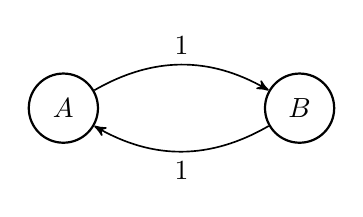
\begin{tikzpicture}[->, >=stealth', auto, semithick, node distance=3cm]
	\tikzstyle{every state}=[fill=white,draw=black,thick,text=black,scale=1]
	\node[state]    (A)               {$A$};
	\node[state]    (B)[right of=A]   {$B$};
	\path
	(A) edge[bend left]			node{$1$}	(B)
	(B) edge[bend left,below]	node{$1$}	(A);
	%\node[above=0.5cm] (A){Patch G};
	%\draw[red] ($(D)+(-1.5,0)$) ellipse (2cm and 3.5cm)node[yshift=3cm]{Patch H};
	\end{tikzpicture}
\end{center}

\textbf{Beispiel:}
\(
    P = \begin{pmatrix}
        1-p & p/2 & p/2\\
        1 & 0 & 0\\
        1 & 0 & 0
    \end{pmatrix}
\) ist aperiodisch für \(p\in [0,1)\), da bei \(p=1\) immer von Zustand 1 in 2 oder 3 gesprungen wird und wieder zurück.
Für alle anderen Werte wird in zwei Fällen auch hin- und zurückgesprungen. Allerdings gibt es auch die Möglichkeit, dass vom
Zustand \(A\) nicht geswechelt wird und man dort bleibt.\\

\begin{center}
	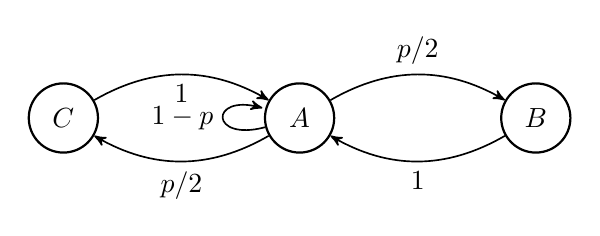
\begin{tikzpicture}[->, >=stealth', auto, semithick, node distance=3cm]
	\tikzstyle{every state}=[fill=white,draw=black,thick,text=black,scale=1]
	\node[state]    (A)               {$A$};
	\node[state]    (B)[right of=A]   {$B$};
	\node[state]    (C)[left of=A]    {$C$};
	% \node[state]    (D)[right of=C]   {$3$};
	\path
	(A) edge[loop left]			node{$1-p$}	(A)
    (A) edge[bend left]			node{$p/2$}	(B)
	(B) edge[bend left,below]	node{$1$}	(A)
    (A) edge[bend left, below]			node{$p/2$}	(C)
    (C) edge[bend left,below]	node{$1$}	(A);
	%\node[above=0.5cm] (A){Patch G};
	%\draw[red] ($(D)+(-1.5,0)$) ellipse (2cm and 3.5cm)node[yshift=3cm]{Patch H};
	\end{tikzpicture}
\end{center}

\subsection{Stoppzeiten}

Eine Stoppzeit ist eine Zufallsvariable, die das Eintreten eines Ereignisses beschreibt, das von der bisherigen Entwicklung eines stochastischen Prozesses abhängt.\\

z.B. die erste Zeit in der Zustand B oder C erreicht wird; Formal:
\begin{equation*}
	\tau  = \inf\{n \geq 0 | X_n \in \{ B, C\}\}
\end{equation*}

Man beginnt dann im Zeitpunkt \(\tau\) mit einer neuen Markov-Kette; diese ist unabhängig von der bisherigen Entwicklung.\\

\end{document}